% The New Quill Developer's Manual
% Copyright (C) 2025 Jorge Fuertes Alfranca
% Released under the GPL v3 or later licenses
%

\documentclass{report}

% Packages used in this example
\usepackage{graphicx}  % for including images and pdf graphics
\usepackage{microtype} % for typographical enhancements
\usepackage{hyperref}  % for hyperlinks
\usepackage[spanish]{babel} % spanish language
\usepackage[a4paper,top=4.2cm,bottom=4.2cm,left=3.5cm,right=3.5cm]{geometry} % for setting page size and margins

% config
\setlength{\parskip}{1em}

% macros
\newcommand{\tnq}{\textit{The New Quill}}
\newcommand{\ic}[1]{\texttt{#1}}
\newcommand{\la}[1]{\textit{#1}}

% front page
\title{\tnq\\ \large Manual del escritor}
\author{\copyright\ 2025 Jorge Fuertes Alfranca \\ \small Released under the GPL v3 or later licenses}

\begin{document}
\begin{center}
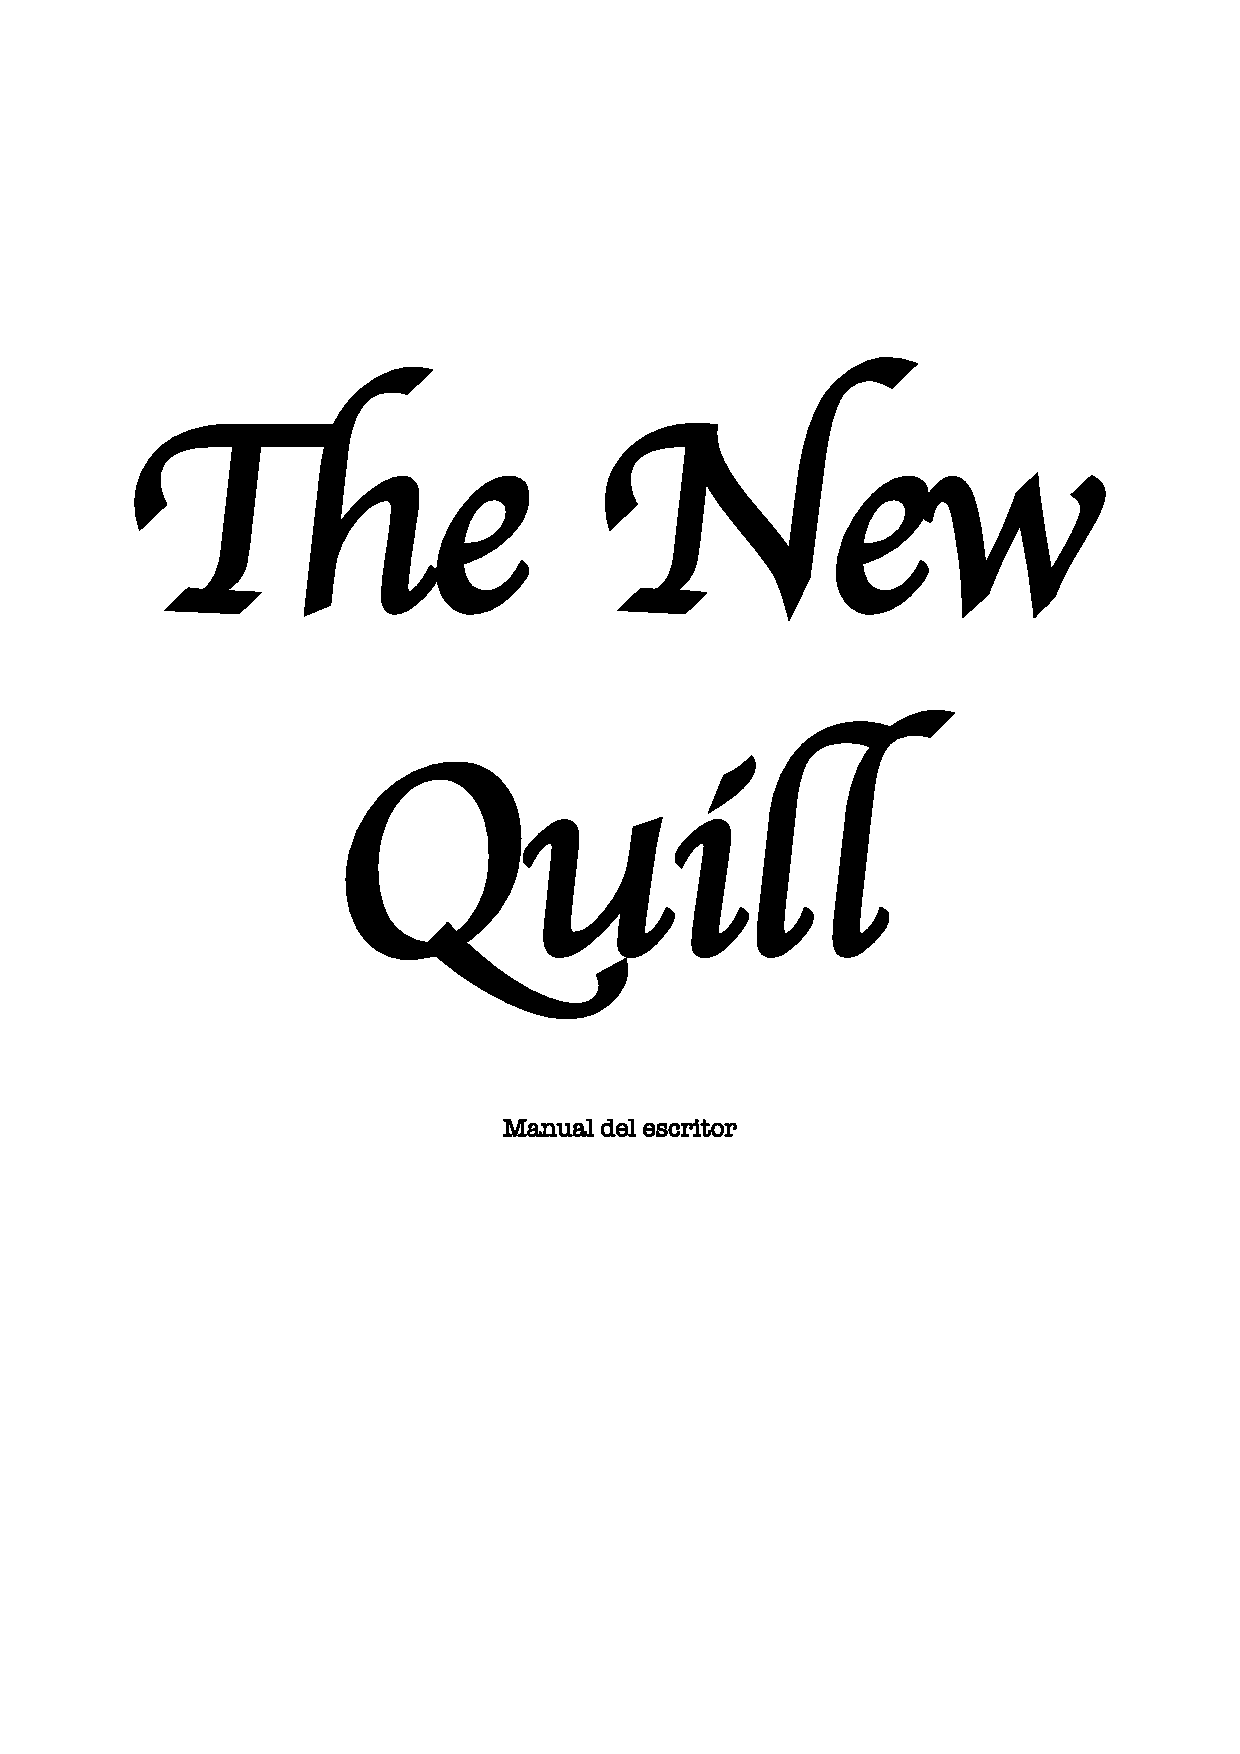
\includegraphics[width=0.98\textwidth]{gfx/portada.pdf}
\end{center}
\newpage

\maketitle
\tableofcontents
\newpage

\chapter{Bienvenida}
    \section{Introducción}
        Bienvenido a \tnq, un sistema de desarrollo de aventuras conversacionales para ordenadores modernos.
        
        Este software están inspirado en los sistemas de desarrollo de aventuras conversaciones de los ochenta,
        especialmente en los de \textit{Gillsoft}, como el programa \textit{PAWS} de \textit{ZX Spectrum} y el
        compilador \textit{DAAD} de PC, además de en todo el trabajo hecho por los pioneros de las aventuras
        conversacionales, con mención especial a la empresa española \textit{Aventuras AD}.

\chapter{El compilador}        
    \section{Línea de comandos}
    \section{Identificadores y etiquetas}
        Cada entidad definida en el código fuente tiene obligatoriamente un identificador y opcionalmente una serie de
        etiquetas. El identificador es único dentro de su clase, es decir, no puede haber dos \ic{items} con \ic{id}
        \la{petaca}, si bien puede haber un objeto con \ic{id} \la{petaca} y una \ic{word} de tipo \ic{noun} con \ic{id}
        \la{petaca}.


\end{document}